\begin{comment}
\begin{itemize}
  \item Room2Room: Enabling Life-Size Telepresence in a Projected Augmented Reality Environment(https://dl.acm.org/doi/pdf/10.1145/2818048.2819965)
  \item Improving visibility of remote gestures in distributed tabletop collaboration(https://dl.acm.org/doi/10.1145/1958824.1958839)
  \item Putting things in focus: establishing co-orientation through video in context(https://dl.acm.org/doi/10.1145/2470654.2466174)
  \item A gaze-preserving group video conference system using screen-embedded cameras(https://dl.acm.org/doi/10.1145/3139131.3141775)
  \item Towards Enabling Eye Contact and Perspective Control in Video Conference (https://dl.acm.org/doi/10.1145/3379350.3416197)
\end{itemize}
\end{comment}
Pejsaら\cite{27}は,投影型の拡張現実環境を用いて,対面時の
ような1対1の遠隔会議が出来るシステムを考案した.Kinnectによって
参加者の動きや体勢を認識して,3Dモデルを自動生成して,相手の
正面へと表示することで,疑似的な対面環境を作り出した.
実験の結果,従来のビデオ会議を用いたコミュニケーションよりも
通信相手の存在感や,コミュニケーションの効率といった観点で
優れていることが示された.一方で,解像度の低さなどの問題から
,ジェスチャーを用いたコミュニケーションの頻度が低下したことや,
1対1のケースに用途が限られている等の問題点が指摘されている.
\begin{figure}[tp]
  \centering
  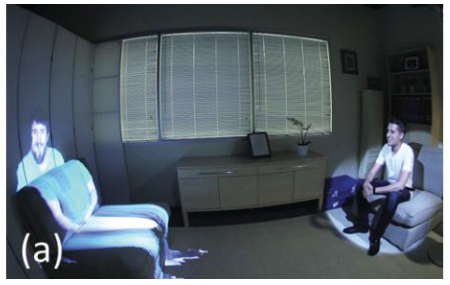
\includegraphics[scale=1.2]{fig/2room2.png}
  \caption{Room2Roomによる通信の様子\cite{27}}
\end{figure}

Yamashitaら\cite{28}は,卓上での作業における遠隔ビデオ会議
において,ジェスチャーの情報が失われることを指摘し,卓上
において遠隔参加者のジャスチャーが視認できるシステムt-Roomを
提案した.卓上ディスプレイに遠隔地参加者のジェスチャーを表示する
際には,物体にさえぎられるなどの問題がある.そこで,リモートラグと呼ばれる
,遠隔地参加者の遅延した映像をリアルタイム映像と同時に表示することで,
ジェスチャーの理解の正誤判断を行えるようにした.
通常表示条件とリモートラグ表示条件での比較実験の結果,ユーザーは
見落としたジェスチャーの情報などを後から再認識することに成功し,ジェスチャー
を見落とすことによる不要な会話が減少したことが示されている.また,作業参加者の
体感作業負荷を減少させたことも示されている.

\begin{figure}[tp]
  \centering
  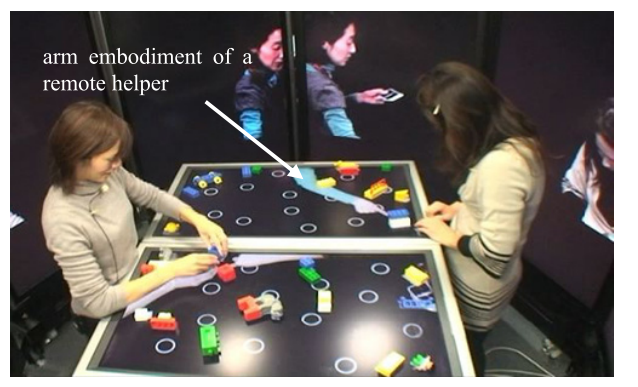
\includegraphics[scale=0.7]{fig/tRoom.png}
  \caption{t-Roomを使用する様子\cite{27}}
\end{figure}

\begin{figure}[tp]
  \centering
  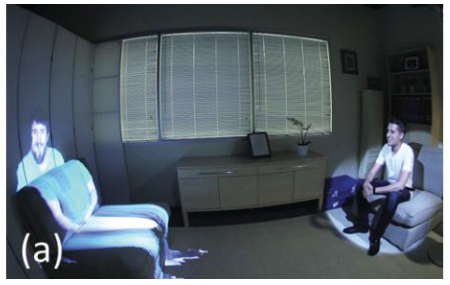
\includegraphics[scale=1.0]{fig/2room2.png}
  \caption{t-Roomの構成\cite{27}}
\end{figure}

Kobayashiら\cite{29}は,Kinnectと,複数のカメラから視線方向の推定を行い,
リアルタイムで,対面時の会話と同じ景色を再現する映像表示方法を提案した.(図\ref{Kobayashi})
Kobayashiらは,2対2でのコミュニケーションを行うケースを想定しており,以下の
場合について表示方法の切り替えを行った.
\begin{itemize}
  \item 一方の側の人物が他方の側のユーザに見られていない場合は,デフォルトの視点位置を使用する.
  \item  一方の面の人物が他方のユーザからのみ見られている場合は,そのユーザの視点位置を使用する.
  \item  一方の面の人物が他方の面の複数のユーザから見られている場合は,お互いを見ているペアを使用する.
\end{itemize}

\begin{figure}[tp]
  \centering
  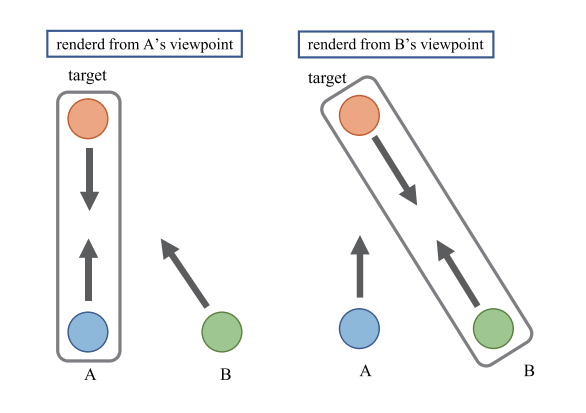
\includegraphics[scale=0.8]{fig/gaze.png}
  \caption{Kobayashiらの提案\cite{29}}\label{Kobayashi}
\end{figure}

\begin{figure}[tp]
  \centering
  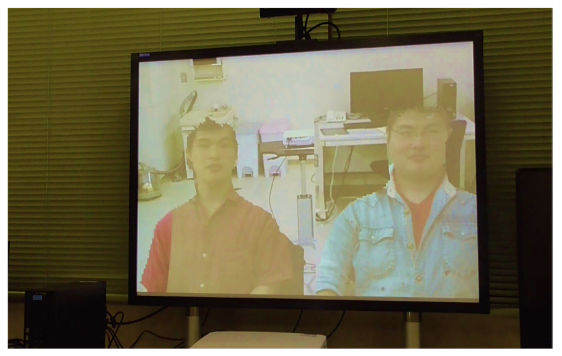
\includegraphics[scale=0.8]{fig/kobayashi2.png}
  \caption{Kobayashiらの提案システムのデモンストレーション\cite{29}}
\end{figure}



